
\begin{frame}\frametitle{There was a time when ``computers'' were humans}
  
  \begin{minipage}{0.45\textwidth}
    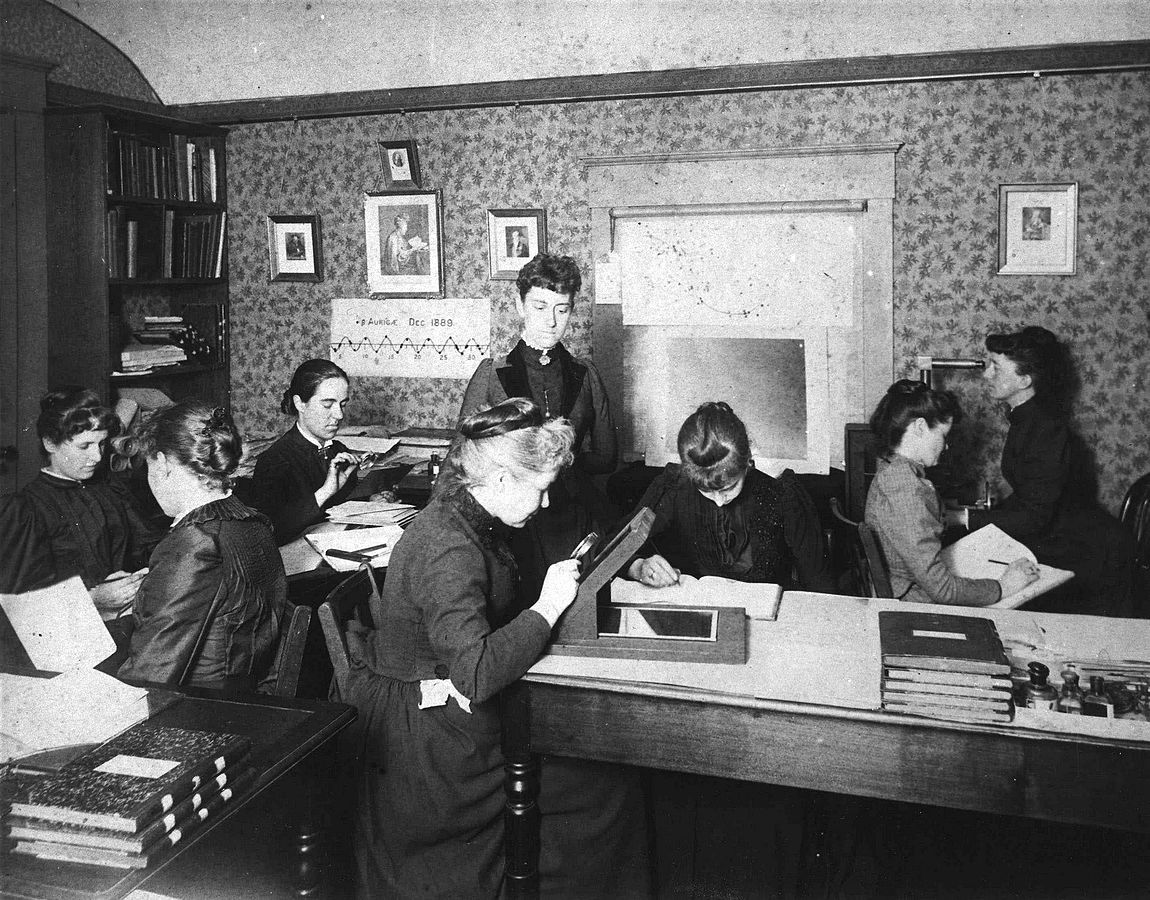
\includegraphics[width=\textwidth]{pic/HarvardComputers.jpg}\newline
    Harvard Computers, circa 1890\newline
    {\tiny By Harvard College Observatory - Public Domain}\newline
    {\tiny \url{https://commons.wikimedia.org/w/index.php?curid=10392913}}
  \end{minipage}\hfill
  \begin{minipage}{0.45\textwidth}
    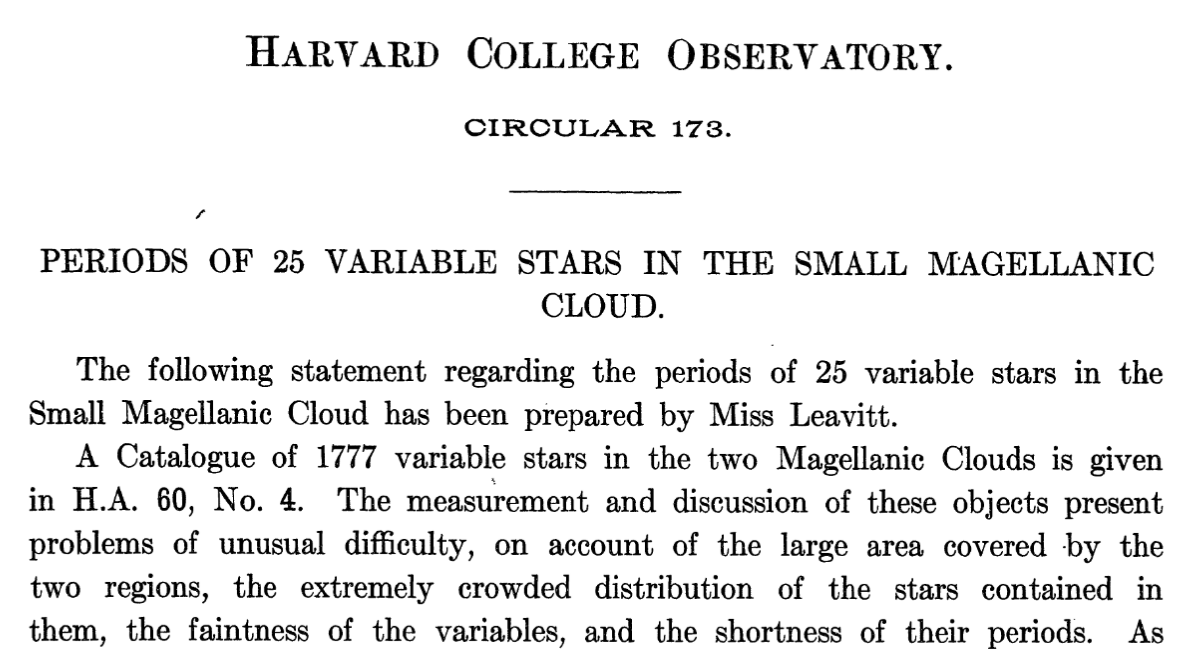
\includegraphics[width=\textwidth]{pic/harvardobs.jpg}
    \vspace{1.25cm}
    It was about science -- astronomy
  \end{minipage}

  Computations of course have been performed since ancient times. One can 
  trace back the termin ``computer'' applied to humans at least until 1613. 
  \only<article>{
    The reference is R. Brathwaite, The Yong Mans Gleanings, London 2014,
    full text available: \url{https://quod.lib.umich.edu/e/eebo/A00514.0001.001?rgn=main;view=fulltext}
  }

  The ``Harvard computers'' became very famous in this context. Incidently, they were
  mostly female. They predate the NASA human computers of recent movie fame.
  \only<article>{See \url{https://en.wikipedia.org/wiki/Harvard_Computers}}

\end{frame}


\begin{frame}\frametitle{Does this scale ?}
  
  \begin{minipage}{0.45\textwidth}
    
\includegraphics[width=\textwidth]{pic/richardsbook}
    \vspace{1.25cm}
    
    L.F.Richardson 1922
  \end{minipage}\hfill
  \begin{minipage}{0.45\textwidth}
    \includegraphics[width=\textwidth]{pic/weatherfactory.jpg}
    
    64000 computers predicting weather (1986 Illustration of L.F. Richardson's vision
    by S. Conlin)
  \end{minipage}
  
  \begin{itemize}
    \tightlist
  \item
    This was about weather, not science in the first place
  \item
    Science \emph{and} Engineering need computing
  \end{itemize}
  
\end{frame}
%%%%%%%%%%%%%%%%%%%%%%%%%%%%%%%%%%%%%%%%%%%%%%%%%%%%%%%%%%%%%%%%%%% 

%%%%%%%%%%%%%%%%%%%%%%%%%%%%%%%%%%%%%%%%%%%%%%%%%%%%%%%%%%%%%%%%%%% 
\begin{frame}\frametitle{Computing was taken over by machines}

  \begin{center}
    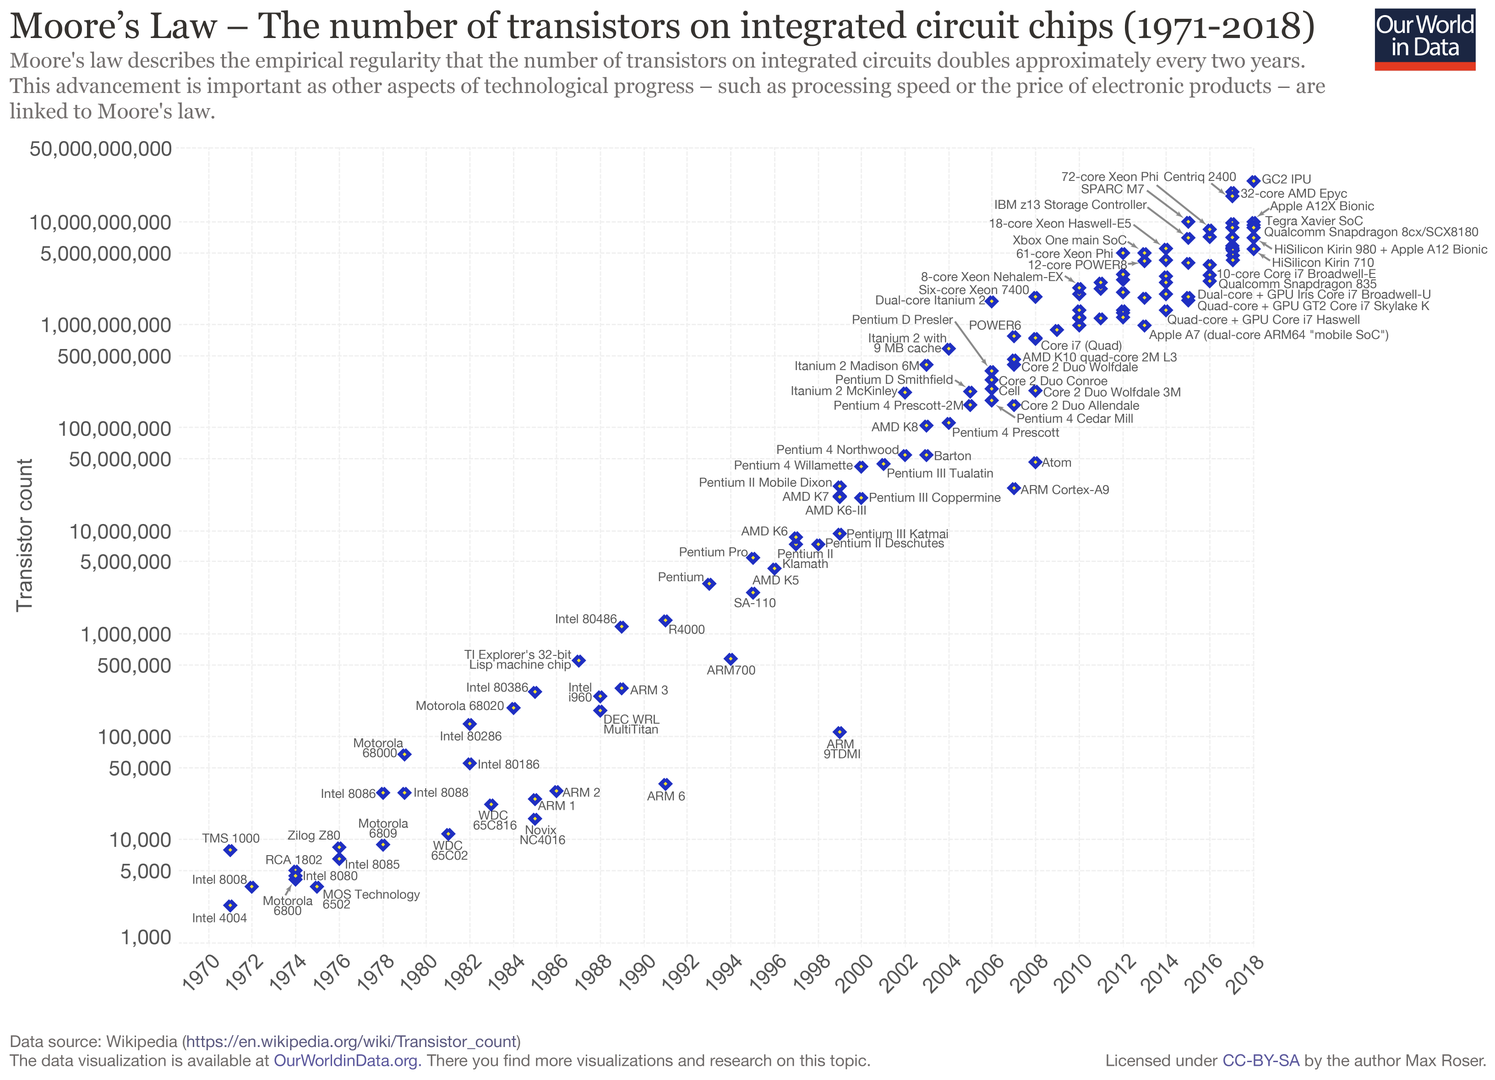
\includegraphics[width=0.95\textwidth]{pic/moore.png}
    \vspace{-0.15cm}

    {\tiny By Max Roser - https://ourworldindata.org/uploads/2019/05/Transistor-Count-over-time-to-2018.png, CC BY-SA 4.0, https://commons.wikimedia.org/w/index.php?curid=79751151}
  \end{center}

\end{frame}
%%%%%%%%%%%%%%%%%%%%%%%%%%%%%%%%%%%%%%%%%%%%%%%%%%%%%%%%%%%%%%%%%%% 

%%%%%%%%%%%%%%%%%%%%%%%%%%%%%%%%%%%%%%%%%%%%%%%%%%%%%%%%%%%%%%%%%%% 
\begin{frame}\frametitle{Computational engineering}

  \begin{itemize}
  \item
    Starting points: Nuclear weapons + rocket design, ballistic
    trajectories, weather \ldots{}
  \item
    Now ubiquitous:

    \begin{itemize}
      \tightlist
    \item
      Structural engineering
    \item
      Car industry
    \item
      Oil recovery
    \item
      Semiconductor design
    \item
      \ldots{}
    \end{itemize}
  \item
    Use of well established, verfied, well supported commercial codes

    \begin{itemize}
      \tightlist
    \item
      Comsol
    \item
      ANSYS
    \item
      Eclipse
    \item
      \ldots{}
    \end{itemize}
  \end{itemize}

\end{frame}
%%%%%%%%%%%%%%%%%%%%%%%%%%%%%%%%%%%%%%%%%%%%%%%%%%%%%%%%%%%%%%%%%%% 

%%%%%%%%%%%%%%%%%%%%%%%%%%%%%%%%%%%%%%%%%%%%%%%%%%%%%%%%%%%%%%%%%%% 
\begin{frame}\frametitle{As soon as computing machines became available \ldots{}}

  \ldots{} Scientists ``misused'' them to satisfy their curiosity

  \begin{minipage}{0.35\textwidth}
    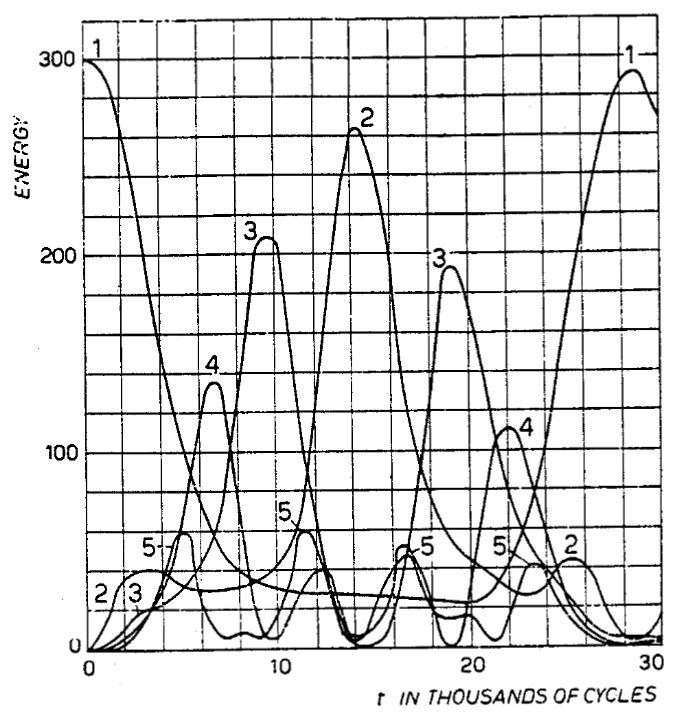
\includegraphics[width=\textwidth]{pic/fpupic}
  \end{minipage}\hfill
  \begin{minipage}{0.6\textwidth}
    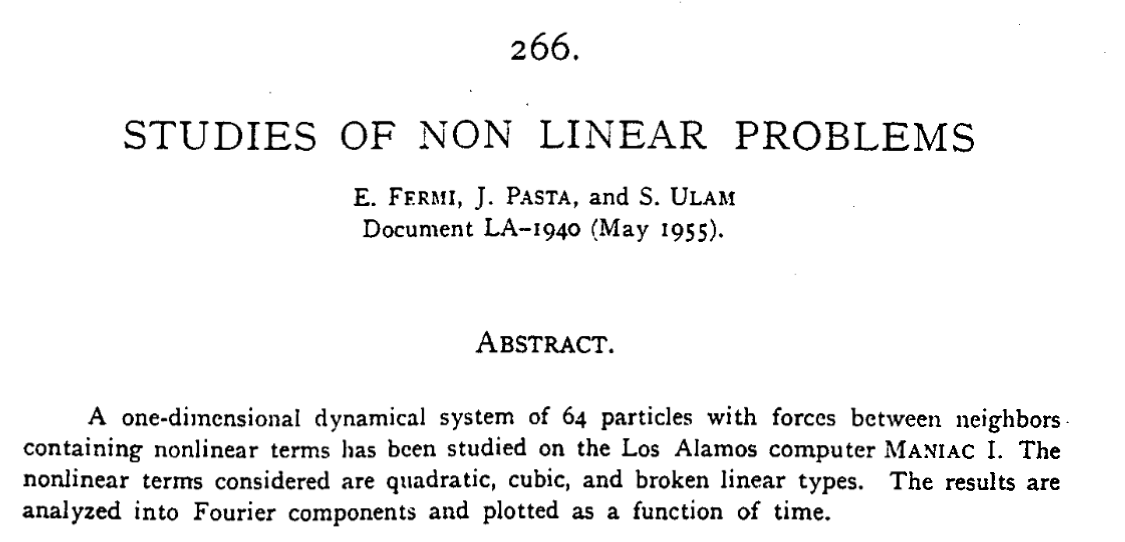
\includegraphics[width=\textwidth]{pic/fputitle}
  \end{minipage}


  ``\ldots{} Fermi became interested in the development and potentialities
  of the electronic computing machines. He held many discussions
  {[}\ldots{}{]} of the kind of future problems which could be studied
  through the use of such machines.''

  Fermi,Pasta and Ulam studied particle systems with \emph{nonlinear}
  interactions

  Calculations were done on the MANIAC-1 computer at Los Alamos

\end{frame}
%%%%%%%%%%%%%%%%%%%%%%%%%%%%%%%%%%%%%%%%%%%%%%%%%%%%%%%%%%%%%%%%%%% 

%%%%%%%%%%%%%%%%%%%%%%%%%%%%%%%%%%%%%%%%%%%%%%%%%%%%%%%%%%%%%%%%%%% 
\begin{frame}\frametitle{And they still do\ldots{}}

  \begin{minipage}{0.45\textwidth}
    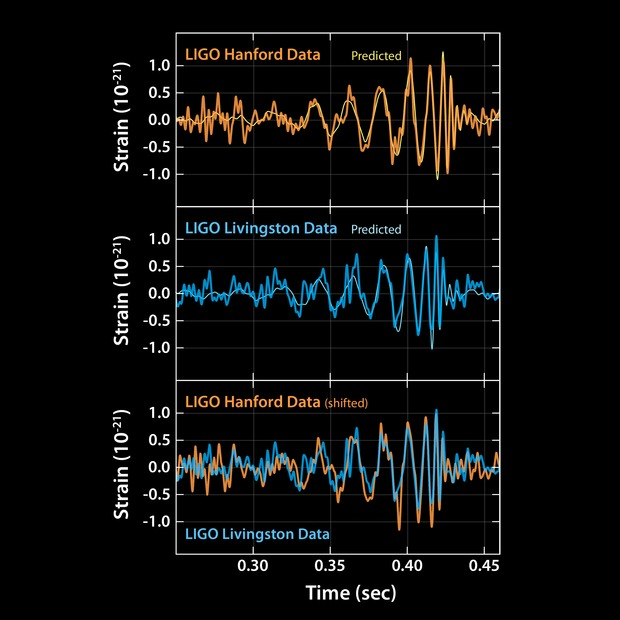
\includegraphics[width=\textwidth]{pic/ligo20160211a.jpg}
    
    
    {\tiny Caltech/MIT/LIGO Lab }
  \end{minipage}\hfill
  \begin{minipage}{0.45\textwidth}
    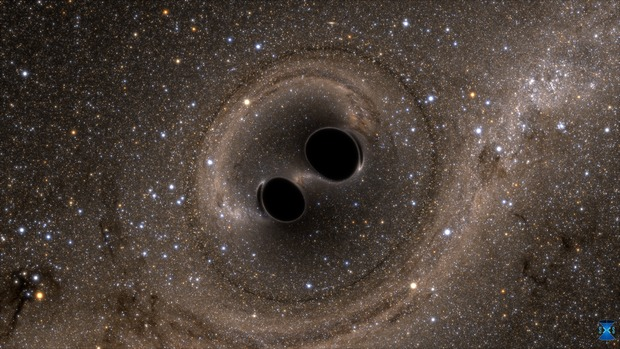
\includegraphics[width=\textwidth]{pic/ligo20160211d.jpg}
    
    
    {\tiny SXS, the Simulating eXtreme Spacetimes (SXS) project (\url{http://www.black-holes.org})}
  \end{minipage}
  
  Verification of the detection of gravitational waves by numerical
  solution of Einstein's equations of general relativity using the
  ``Spectral Einstein Code''

  Computations significantly contributed to the 2017 Nobel prize in physics
\end{frame}
%%%%%%%%%%%%%%%%%%%%%%%%%%%%%%%%%%%%%%%%%%%%%%%%%%%%%%%%%%%%%%%%%%% 

%%%%%%%%%%%%%%%%%%%%%%%%%%%%%%%%%%%%%%%%%%%%%%%%%%%%%%%%%%%%%%%%%%% 
\begin{frame}\frametitle{Scientific computing}

  \textbf{``The purpose of computing is insight, not numbers.''}\\
  (\url{https://en.wikiquote.org/wiki/Richard_Hamming})

  \begin{itemize}
    \tightlist
  \item
    Frontiers of Scientific Computing

    \begin{itemize}
      \tightlist
    \item
      Insight into complicated phenomena not accessible by other methods
    \item
      Improvement of models to better fit reality
    \item
      Improvment of computational methods
    \item
      Generate testable hypothesis
    \item
      Support experimentation in other scientific fields
    \item
      Exploration of new computing capabilities
    \item
      Prediction, optimization of complex systems
    \end{itemize}
  \item
    Good scientifc practice

    \begin{itemize}
      \tightlist
    \item
      Reproducibility
    \item
      Sharing of ideas and knowledge
    \end{itemize}
  \item
    Interdisciplinarity

    \begin{itemize}
      \tightlist
    \item
      Numerical Analysis
    \item
      Computer science
    \item
      Modeling in specific fields
    \end{itemize}
  \end{itemize}

\end{frame}
%%%%%%%%%%%%%%%%%%%%%%%%%%%%%%%%%%%%%%%%%%%%%%%%%%%%%%%%%%%%%%%%%%% 

%%%%%%%%%%%%%%%%%%%%%%%%%%%%%%%%%%%%%%%%%%%%%%%%%%%%%%%%%%%%%%%%%%% 
\begin{frame}\frametitle{General approach}

  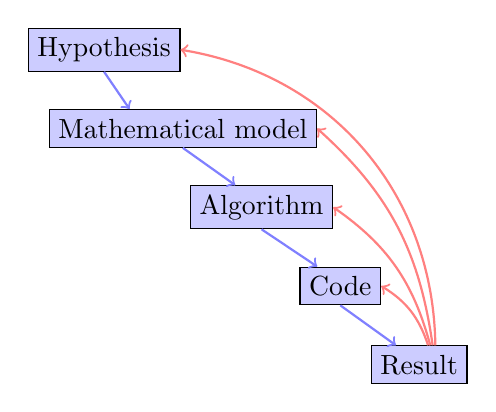
\begin{tikzpicture}
    \node (Hyp) at (2,4) [fill=blue!20,draw] {Hypothesis};
    \node (Mod) at (3,3) [fill=blue!20,draw] {Mathematical model};
    \node (Alg) at (4,2) [fill=blue!20,draw] {Algorithm};
    \node (Cod) at (5,1) [fill=blue!20,draw] {Code};
    \node (Res) at (6,0) [fill=blue!20,draw] {Result};


    \draw[->, blue!50, thick] (Hyp.south) to (Mod.160);
    \draw[->, blue!50, thick] (Mod.south) to (Alg.140);
    \draw[->, blue!50, thick] (Alg.south) to (Cod.140);
    \draw[->, blue!50, thick] (Cod.south) to (Res.140);
    \draw[->, red!50, thick] (Res.65) to[bend right=20] (Cod.east);
    \draw[->, red!50, thick] (Res.60) to[bend right=20] (Alg.east);
    \draw[->, red!50, thick] (Res.55) to[bend right=20] (Mod.east);
    \draw[->, red!50, thick] (Res.50) to[bend right=40] (Hyp.east);
  \end{tikzpicture}

  \begin{itemize}
    \tightlist
  \item
    Possible (probable) involvement of different persons, institutions
  \item
    It is important to keep interdisciplinarity in mind
  \end{itemize}

\end{frame}
%%%%%%%%%%%%%%%%%%%%%%%%%%%%%%%%%%%%%%%%%%%%%%%%%%%%%%%%%%%%%%%%%%% 

%%%%%%%%%%%%%%%%%%%%%%%%%%%%%%%%%%%%%%%%%%%%%%%%%%%%%%%%%%%%%%%%%%% 
\begin{frame}\frametitle{Scientific computing tools}

  Many of them are Open Source

  \begin{itemize}
    \tightlist
  \item
    General purpose environments

    \begin{itemize}
      \tightlist
    \item
      Matlab
    \item
      COMSOL
    \item
      Python + ecosystem
    \item
      R + ecosystem
    \item
      \textbf{Julia}
    \end{itemize}
  \item
    ``Classical'' computer languages + compilers

    \begin{itemize}
      \tightlist
    \item
      Fortran
    \item
      C, C++
    \end{itemize}
  \item
    Established special purpose libraries

    \begin{itemize}
      \tightlist
    \item
      Linear algebra: LAPACK, BLAS, UMFPACK, Pardiso
    \item
      Mesh generation: \textbf{triangle}, TetGen, NetGen
    \item
      Eigenvalue problems: ARPACK
    \item
      Visualization libraries: VTK
    \end{itemize}
  \item
    Tools in the ``background''

    \begin{itemize}
      \tightlist
    \item
      Build systems Make, CMake
    \item
      Editors + IDEs (emacs, jedit, eclipse, atom, Visual Studio Code)
    \item
      Debuggers
    \item
      Version control (svn, \textbf{git}, hg)
    \end{itemize}
  \end{itemize}

\end{frame}

\begin{frame}\frametitle{Confusio Linguarum}

  \begin{minipage}{0.45\textwidth}
    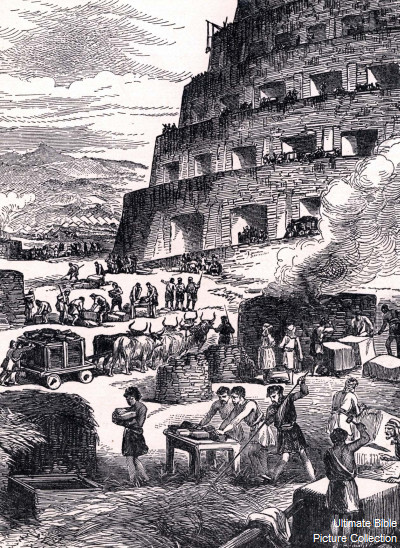
\includegraphics[width=\textwidth]{pic/Babel_1166-12.jpg}
  \end{minipage}\hfill
  \begin{minipage}{0.45\textwidth}
    "And   the  whole   land   was   of  one   language   and  of   one
    speech. ...  And they said, Go to, let us build  us a city and a
    tower whose top may  reach unto heaven. ...  And the Lord said,
    behold,   the   people   is   one,   and   they   have   all   one
    language. ... Go to, let  us go down, and  there confound their
    language that  they may not  understand one another’s  speech.  So
    the Lord  scattered them abroad from  thence upon the face  of all
    the earth." (Daniel 1:1-7)
  \end{minipage}

\end{frame}
%%%%%%%%%%%%%%%%%%%%%%%%%%%%%%%%%%%%%%%%%%%%%%%%%%%%%%%%%%%%%%%%%%% 

%%%%%%%%%%%%%%%%%%%%%%%%%%%%%%%%%%%%%%%%%%%%%%%%%%%%%%%%%%%%%%%%%%% 
\begin{frame}\frametitle{Once again Hamming}

  \ldots{}of ``Hamming code'' and ``Hamming distance'' fame, who started
  his carrier programming in Los Alamos:

  ``Indeed, one of my major complaints about the computer field is that
  whereas Newton could say,''If I have seen a little farther than others,
  it is because I have stood on the shoulders of giants," I am forced to
  say, ``Today we stand on each other's feet.'' Perhaps the central
  problem we face in all of computer science is how we are to get to the
  situation where we build on top of the work of others rather than
  redoing so much of it in a trivially different way. Science is supposed
  to be cumulative, not almost endless duplication of the same kind of
  things." (1968)

  \begin{itemize}
    \tightlist
  \item
    2017 this is still a problem
  \end{itemize}

\end{frame}
%%%%%%%%%%%%%%%%%%%%%%%%%%%%%%%%%%%%%%%%%%%%%%%%%%%%%%%%%%%%%%%%%%% 

%%%%%%%%%%%%%%%%%%%%%%%%%%%%%%%%%%%%%%%%%%%%%%%%%%%%%%%%%%%%%%%%%%% 
\begin{frame}\frametitle{Intended  aims  and topics of this course}

  \begin{itemize}
  \item
    Indicate a reasonable path within this labyrinth
  \item
    Introduction to  Julia
  \item
    Software management skills (version control)
  \item
    Relevant topics from numerical analysis
  \item
    Focus on partial differential equation (PDE) solution
    \begin{itemize}
      \tightlist
    \item Solution of large linear systems of equations
    \item
      Finite elements
    \item
      Finite volumes
    \item
      Mesh generation
    \item
      Linear and nonlinear solvers
    \item
      Parallelization
    \item
      Visualization
    \end{itemize}
  \end{itemize}

\end{frame}

%%% Local Variables:
%%% mode: latex
%%% TeX-master: "l01-intro"
%%% End:
